\documentclass{article}
\usepackage[english]{babel}
\usepackage[utf8]{inputenc}

% Graphics package
\usepackage{graphicx}
\graphicspath{ {images/} }

%Includes "References" in the table of contents
\usepackage[nottoc]{tocbibind}


% Latex commands
    \newcommand{\mat}[2][ccccccccccccccccccccccccccccccccccccccccccccc]{\left[
        \arraycolsep=1.2pt\def\arraystretch{1.5}
        \begin{array}{#1} #2 \\ 
        \end{array} 
        \right]}

        %% Miscelaneous commands
        
        %% Tool tracking positions
        \newcommand{\xbT}{\bf{x}{^b_T}} % tool tip in body coords
        \newcommand{\xwT}{\bf{x}{^w_T}} % tool tip in world coords
        \newcommand{\xcT}{\bf{x}{^c_T}} % tool tip in camera coords
        \newcommand{\xwE}{\bf{x}{^w_E}} % eraser in world coords
        \newcommand{\xcE}{\bf{x}{^c_E}} % eraser in camera coords

        \newcommand{\obT}{\bf{\theta}{^b_T}} % eraser in camera coords

        %% Tool tracking orientations
        \newcommand{\q}[3]{{^#1}\bf{q}{^#2_#3}} % eraser in world coords

        %% Rotation and Translation vectors
        \newcommand{\R}[2]{{^#1}{\bf{R}}{^#2}}
        \newcommand{\T}[2]{{^#1}{\bf{t}}{^#2}}

        \newcommand{\tab}{\text{ \ \ \ \ }}


\begin{document}

\title{Final Progress Report}
\author{Lukas Gemar}
\date{March 4, 2016}
\maketitle

\begin{flushleft}

%%%%%%%%%%%%%%%%%%%%%%%%%%%%%%%%%%%%%%%%%%%%%%%%%%%%%%%%%%%%%%%%%%%%%%%%%%%%%%%
%%%%% Tool Model
%%%%%%%%%%%%%%%%%%%%%%%%%%%%%%%%%%%%%%%%%%%%%%%%%%%%%%%%%%%%%%%%%%%%%%%%%%%%%%%
\section{Tool Model}

\medskip

The position of the tip of the interaction tool is $ \xwT $. This position is specified in world coordinates; the superscript $w$ indicates that the coordinates of this position are specified relative to the origin of world space, $\bf{O_w}$. This origin of the world coordinate system is approximately the location of the users head. It is not exactly the location of the user's head because the user can look up and down and side to side while wearing the display. The origin of the world coordinate system should remain fixed to these rotations and translations. The rotation of the display is measured, but the translation of the display is not. However, the translation of the head should be a function of the rotation of the display. A simple model of how the head moves from side to side should relate the head's rotation to its movement relative to the neck and shoulders.

\medskip

Since the camera is mounted to the display, the position of the world coordinate system is not exactly the position of the camera. The origin of the camera coordinate system, $\bf{O_c}$, is offset from the world coordinate system by the rotation and translation of the user's head. Assuming that the rotation and translation of the user's head is in fact minimal while the user is seated, then the translation of the camera, $\T{c}{w}$, should be a function of the rotation of the head mounted display, $\R{c}{w}$: $\T{c}{w} = f(\R{c}{w})$. 

\medskip

Let $\R{c}{w}$ and $\T{c}{w}$ be the rotation and translation matrices, respectively, that specify the transformation from the world coordinate system to the camera coordinate system. Then the position of the interaction tool in camera coordinates, $ \xcT $,  is given by the following relation: 

\[ \xcT = \R{c}{w} \xwT + \T{c}{w} \]

The position of the tool relative to the camera, $ \xcT $, is not observed directly. However, this position is inferred from the position of the back of the tool, $ \xcE $, and the orientation of the tool. Call the back of the tool the eraser. The position of the eraser, $\xcE$, is found through computer vision. The orientation of the tool relative to the world coordinate systsem is specified by the orientation of the tool in body coordinates, $\obT$, and the rotation matrix from the body coordinates of the tool to the world coordinates, $\R{w}{b}$; their product yields the absolute orientation of the tool in world coordinates. To correctly display the orientation of the tool to the user, $\R{w}{b}$, the rotation of the camera relative to the world, must also be known. $\R{w}{b}$ is measured by the virtual reality display. The position of the tool in camera coordiantes is found through the following relation: 

\[ \xcT = \xcE + \R{c}{w}(\R{w}{b}\obT) \]

\medskip
%%%%%%%%%%%%%%%%%%%%%%%%%%%%%%%%%%%%%%%%%%%%%%%%%%%%%%%%%%%%%%%%%%%%%%%%%%%%%%%
%%%%% Camera Model
%%%%%%%%%%%%%%%%%%%%%%%%%%%%%%%%%%%%%%%%%%%%%%%%%%%%%%%%%%%%%%%%%%%%%%%%%%%%%%%
\section{Camera Model}

The following is a model of a single frame from the camera. In this frame, the red circular object represents the back of the interaction tool. The back of the interaction tool is called the eraser. The width of the target along the $x$ dimension of the image is $d_{u}$. 

\medskip

\begin{center}
    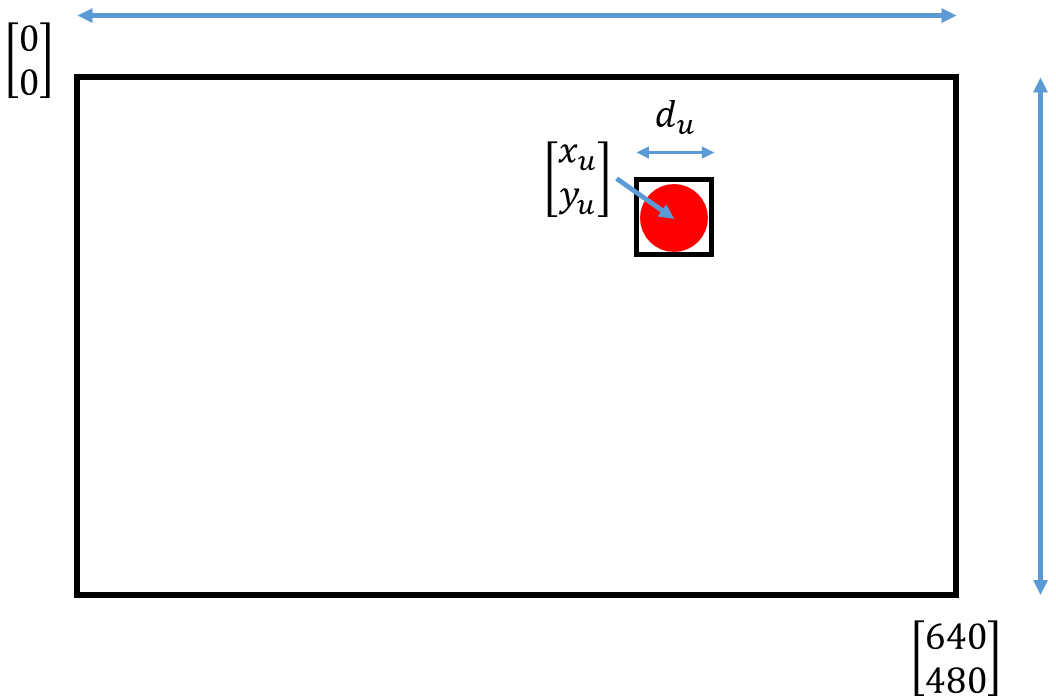
\includegraphics[scale=0.4]{computerVision}
\end{center}

\medskip

The midpoint of the eraser in the ideal undistorted image is $\bf{x^u_E} = \mat{ x_u & y_u }^{T}$. The center of the undistorted image is $c_x$ in the x direction and $c_y$ in the y direction. The focal lengths in the x and y directions are $f_x$ and $f_y$, respectively. These parameters are found through the camera calibration routine. The measurements of the center of the eraser and its width are related to the hidden state $\bf{\bf{x_C}} = \mat{ x_C & y_C & z_C }^{T}$ in the following way: 

\[
    \bf{\bf{y}} = h(\bf{\bf{x}})
        = \mat{x_u \\ y_u \\ d_{u} }
        = \mat{ \frac{f_x x_c}{z_c} + c_x \\ 
             \frac{f_y y_c}{z_c} + c_y \\ 
             \frac{d_c}{z_c \sqrt{\frac{1}{f_x^{2}} + \frac{1}{f_y^{2}}}}
           }
\]

These relationships are found through using a simple pin-hole camera model \cite{Tsai1987}.

%%%%%%%%%%%%%%%%%%%%%%%%%%%%%%%%%%%%%%%%%%%%%%%%%%%%%%%%%%%%%%%%%%%%%%%%%%%%%%%
%%%%% Attitude Estimation
%%%%%%%%%%%%%%%%%%%%%%%%%%%%%%%%%%%%%%%%%%%%%%%%%%%%%%%%%%%%%%%%%%%%%%%%%%%%%%%
\section{Attitude Estimation}

The attitude of the interaction tool relative to the world coordinate frame can be represented in a number of ways. The two representations that will be important here are the attitude matrix and the attitude quaternion. First, the attitude of the orientation tool can be described by the attitude matrix $A$. The attitude matrix typically maps a vector in the reference frame to a vector in the the body frame \cite{Markley2007}. This mapping is given by the relation, 

\[ \bf{b} = A \bf{r} \]

Second, the attitude of the interaction tool can be represented as a quaternion. A rotation in three-dimensions is equivalent to an axis of rotation and and angle of rotation. If $\hat{n}$ is the axis of a rotation and $\theta$ is the angle of the rotation, then the quaternion $\overline{q}$ represents the attitude: 

\[ \overline{q} = \mat{\vec{q} \\ q_4} \] 

with $\vec{q} = \hat{n} \sin{\frac{\theta}{2}}$ and $q_4 = \cos{\frac{\theta}{2}}$. The quaternion must have length 1: $\overline{q}^T \overline{q} = 1$. 

The attitude matrix and the quaternion representing attitude are related by the following equation, where $A$ is a function of $\overline{q}$ \cite{Shuster1982}: 

\[ A(\overline{q}) = (q_4^2 - {\| \vec{q} \|}^2) I_{3x3} + 2 \vec{q}\vec{q}^T - 2 q_4 [\vec{q}\times] \]

where ${[\vec{q}\times}]$ is the skew-symmetric cross product matrix, 

\[ [\vec{q}\times] = \mat{ 0 & -q_3 & q_2 \\ q_3 & 0 & -q_1 \\ -q_2 & q_1 & 0} \]

The relationship between $A$ and $\overline{q}$ can also be expressed as the product of two matrices \cite{Markley2007}: 

\[ A(\overline{q}) = \Xi(\overline{q})^{T} \Psi(\overline{q}) \]

with 

\[ \Xi(\overline{q}) = \mat{q_4 \bf{I}_{3x3} + [\vec{q}\times] \\ -\vec{q}^T } \]

\[ \Psi(\overline{q}) = \mat{q_4 \bf{I}_{3x3} - [\vec{q}\times] \\ -\vec{q}^T } \]

\subsection{Deterministic Attitude Determination}

The TRIAD algorithm finds the attitude matrix $A$ that maps three reference frame vectors $\vec{r}_k$ to their corresponding body frame vectors $\vec{b}_k$ for $k = 1, 2, 3$ \cite{Shuster2004}. Two observations of reference frame vectors provide sufficient information to compute a right-handed orthonormal triad of vectors in the reference frame. If $\vec{v}_1$ and $\vec{v}_2$ are reference frame vectors for the accelerometer and the magnetometer, respecitively, then 

$$ \vec{v}_1 = \mat{ 0 & 0 & 1 }^{T} \tab \text{and} \tab \vec{v}_2 = \mat{ 18006 & -1566 & 53490 }^{T} $$ 

so that the gravity vector points down and the magnetometer vector points in the direction of North in Boston. The orthonormal vector triad representing the reference frame is given by, 

$$ \vec{r}_1 = \frac{\vec{v}_1}{\| \vec{v}_1 \|}, \tab \vec{r}_2 = \frac{\vec{v}_1 \times \vec{v}_2}{\| \vec{v}_1 \times \vec{v}_2 \|}, \tab \vec{r}_3 = \vec{r}_1 \times \vec{r}_2 $$

Let $\vec{w}_1$ be the measurement of the normalized unit vector from the accelerometer and $\vec{w}_2$ be the measurement of the normalized unit vector from the magnetometer, then the orthonormal vector triads for the reference vectors are given by, 

$$ \vec{b}_1 = \frac{\vec{w}_1}{\| \vec{w}_1 \|}, \tab \vec{b}_2 = \frac{\vec{w}_1 \times \vec{w}_2}{\| \vec{w}_1 \times \vec{w}_2 \|}, \tab \vec{b}_3 = \vec{w}_1 \times \vec{w}_2 $$

If there was no noise in the system, then it would be the case that $\vec{b}_k = A \vec{r}_k$ for $k=1,2,3$. An equivalent way of writing this in matrix form is the following: 

$$ M_b = A M_r $$ 

where 

$$ M_b = \mat{ \vec{b}_1 & \vec{b}_2 & \vec{b}_3 } $$
$$ M_r = \mat{ \vec{r}_1 & \vec{r}_2 & \vec{r}_3 } $$

Since $M_r$ is an orthogonal matrix, its inverse is equal to its transpose: $M_r^{-1} = M_r^{T}$. Thus, the solution for the attitude matrix is, 

$$ A = M_b M_r^{T} $$

\subsection{Dynamic Model for Rotations}

The rate of change of the attitude can be written in the form of a general state space model: 

\[ \dot{\vec{x}} = A(\vec{x}, t) \vec{x} + B(\vec{x}, t) \vec{u} \]

The kinematic equation for the change in attitude as a function of the angular rate can be written as a rate of change of the attitude matrix or a rate of change in the quaternion \cite{Shuster1982}. The angular velocity vector is given by $\vec{\omega}$. The rate of change of the attitude matrix is, 

\[ \dot{A}(t) = [\vec{\omega}\times] A(t) \]

In this equation, $[\vec{\omega}\times]$ is an instance of the state transition matrix $A(\vec{x}, t)$ from the general schema for a state space model. The kinematic relation for the rate of change of the quaternion can be written in the following two ways: 

\[ \dot{\overline{q}} = \frac{1}{2} \Omega( \vec{\omega} ) \overline{q} \]

\[ \dot{\overline{q}} = \frac{1}{2} \Xi( \overline{q} )\vec{\omega} \]

where the first relation is a state space model with state transition matrix $A(\vec{\omega}) = \Omega(\omega)$, where the state transition matrix is a function of the angular rate vector $\vec{\omega}$:

\[ \Omega(\vec{\omega}) = \mat{ -[\vec{\omega}\times] & \vec{w} \\ -\vec{\omega}^T & 0 } \] 

The second kinematic equation for the rate of change of the quaternion is an instance of the schema for the state space model where the angular rate $\vec{\omega}$ is treated as the input $\vec{u}$ to the system and the input matrix $B(\overline{q}) = \Xi(\overline{q})$ is a function of the current attitude $\overline{q}$. 

\medskip

There are two good reasons to use the quaternion representation of attitude: first, the rate of change of the quaternion is linearly related to the state of the quaternion; and second, successive rotations are computed by taking the product of quaternions \cite{Markley2007}. The following identity holds of the composition of quaternions \cite{Shuster1982}: 

\[ A(\overline{q}_1) A(\overline{q}_2) = A(\overline{q}_1 \otimes \overline{q}_2) \]

with the operation $A(\overline{q})$ finding the attitude matrix $A$ that corresponds with the quaternion $\overline{q}$. Following the notation in \cite{Markley2007}, the product of the quaternion is linear in each of the quaternions $\overline{q}_1$ and $\overline{q}_2$: 

\[ \overline{q}_1 \otimes \overline{q}_2 = \mat{ \Psi({\overline{q}_1}) & \overline{q}_1} \overline{q}_2 = \mat{ \Xi({\overline{q}_1}) & \overline{q}_1 } \overline{q}_2 \]

The inverse of the quaternion is found by negating the imaginary component of the quaternion: 

\[ \overline{q}^{-1} = \mat{ -\vec{q} \\ q_4 } \]

\subsection{Kalman Filter Design} 

A discrete dynamical system is described by a process model and measurement model. The estimation problem arises in trying to find the hidden state $x_k$ by observing the measurements $z_k$. In their most general form, the system model and the measurement model are given by the equations, 

\[ x_{k+1} = A x_k + B u_k \]
\[ z_k = H x_k \]

A general estimator or observer is given by the equation \cite{Lewis2007}: 

\[ \hat{x}_{k+1} = A \hat{x}_k + L (z_k - H \hat{x}_k) + B u_k \]

From the dynamic model and the measurement equation, $A$, $B$, and $H$ are known. Therefore, it is only necessary to find the observer gain matrix, $L$. 

\medskip

For the Kalman filter, assume that the the process model and the measurement model are both subject to white noise with zero mean and some covariance. Then the process model and measurement equation become 

\[ x_{k+1} = A x_k + B u_k + G_k w_k \]
\[ z_k = H x_k + v_k \]
\[ x_0 \sim (\overline{x}_0, P_{x0}) \]

where the assumptions are that {$w_k$} and {$v_k$} are uncorrelated white noise processes such that $w_k \sim (0, Q_k)$ and $v_k \sim (0,R_k)$. 

\medskip

The Kalman filter has three steps: (1) initialization, (2) time update, and (3) measurement update. During the intialization phase, the state of the model and the covariance are assigned initial values: 

\[ P_0 = P_{x0}  \ \ \ \  \hat{x}_0 = \overline{x}_0 \]

During the time update, also known as the prediction step, the \textit{a priori} estimates for the state and the covariance matrix are given by the following equations: 

$$ P{^{-}_{k+1}} = A_k P_k A_k^{T} + G_k Q_k G_k^{T} $$
$$ \hat{x}{^{-}_{k+1}} = A_k \hat{k} + B_k u_k $$

The measurement update converts the \textit{a priori} predictions for the state and covariance into their \textit{a posteriori} filtered estimates based on the observation of $z_k$: 

$$ P_{k+1} = [ (P{^{-}_{k+1}})^{-1} + H_{k+1}^{T} R_{k+1}^{-1} H_{k+1} ]^{-1} $$
$$ \hat{x}_{k+1} = \hat{x}{^{-}_{k+1}} + P_{k+1} H_{k+1}^{T} R_{k+1}^{-1} (z_{k+1} - H_{k+1} \hat{x}{^{-}_{k+1}}) $$

Note that during the measurement update, the \textit{a posteriori} estimate is simply the \textit{a priori} estimate plus a correction term. The correction term is simply a gain matrix times the the difference between the actual observation and the predicted observation. The gain matrix is known as the Kalman gain: 

$$ K_k = P_k H_k^{T} R_k^{-1} $$

The difference between the actual observation, $z_{k+1}$ and the predicted observation $H_k \hat{x}{^-_{k+1}}$ is known as the residual, $\nu$:

$$ \nu = z_{k+1} - H_k \hat{x}{^-_{k+1}} $$

Thus, the measurement update can be written in terms of the \textit{a priori} estimate, the residual, and the Kalman gain:

$$ \hat{x}_{k+1} = \hat{x}{^-_{k+1}} + K_k \nu $$

\subsubsection{Process Model}

Treat the angular rate, $\vec{\omega}$, as the input to the process model. The rate of change of the quaternion is given by the dynamic model, 

\[ \dot{\overline{q}} = B(\overline{q}) \vec{\omega} \]

with the input matrix $B(\overline{q})$: 

\[ B(\overline{q}) = \frac{1}{2} \Xi(\overline{q}) = \mat{q_4 \bf{I}_{3x3} + [\vec{q}\times] \\ -\vec{q}^T } \]

Treating the attitude quaternion $\overline{q}$ as roughly constant over a small time interval, the process model can be discretized: 

\[ \overline{q}_{k+1} = B_k(\overline{q}_k) \vec{\omega_k} \]

\subsubsection{Measurement Model}

\subsubsection{Prediction Equations}

The prediction variables are the state of the quaternion at the next time step, $\overline{q}_{k+1}$, and the covariance matrix, $\overline{P}_{k+1}$. The state prediction is computed using the process model: 

\[ \dot{\overline{q}} = B(\overline{q}) \vec{\omega} \]

The covariance prediction is computed 


%%%%%%%%%%%%%%%%%%%%%%%%%%%%%%%%%%%%%%%%%%%%%%%%%%%%%%%%%%%%%%%%%%%%%%%%%%%%%%%
%%%%% Bibliography
%%%%%%%%%%%%%%%%%%%%%%%%%%%%%%%%%%%%%%%%%%%%%%%%%%%%%%%%%%%%%%%%%%%%%%%%%%%%%%%
\bibliographystyle{unsrt}
\bibliography{references}

%%%%%%%%%%%%%%%%%%%%%%%%%%%%%%%%%%%%%%%%%%%%%%%%%%%%%%%%%%%%%%%%%%%%%%%%%%%%%%%
%%%%% End of the document
%%%%%%%%%%%%%%%%%%%%%%%%%%%%%%%%%%%%%%%%%%%%%%%%%%%%%%%%%%%%%%%%%%%%%%%%%%%%%%%

\end{flushleft}
\end{document}

